\documentclass[zavrsnirad]{fer}
% Dodaj opciju upload za generiranje konačne verzije koja se učitava na FERWeb
% Add the option upload to generate the final version which is uploaded to FERWeb


\usepackage{blindtext}


%--- PODACI O RADU / THESIS INFORMATION ----------------------------------------

% Naslov na engleskom jeziku / Title in English
\title{Analysis of basketball training through a mobile application}

% Naslov na hrvatskom jeziku / Title in Croatian
\naslov{Analiza treninga košarke putem mobilne aplikacije}

% Broj rada / Thesis number
\brojrada{1936}

% Autor / Author
\author{Vedran Kumanović}

% Mentor 
\mentor{izv. prof. dr. sc.\@ Matko Orsag}

% Datum rada na engleskom jeziku / Date in English
\date{June, 2025}

% Datum rada na hrvatskom jeziku / Date in Croatian
\datum{lipanj, 2025.}

%-------------------------------------------------------------------------------


\begin{document}


% Naslovnica se automatski generira / Titlepage is automatically generated
\maketitle


%--- ZADATAK / THESIS ASSIGNMENT -----------------------------------------------

% Zadatak se ubacuje iz vanjske datoteke / Thesis assignment is included from external file
% Upiši ime PDF datoteke preuzete s FERWeb-a / Enter the filename of the PDF downloaded from FERWeb
\zadatak{hr_1191247427_73.pdf}


%--- ZAHVALE / ACKNOWLEDGMENT --------------------------------------------------

\begin{zahvale}
  Hvala svima koji su mi pomogli u radu na ovom završnom radu.
  
\end{zahvale}


% Odovud započinje numeriranje stranica / Page numbering starts from here
\mainmatter


% Sadržaj se automatski generira / Table of contents is automatically generated
\tableofcontents


%--- UVOD / INTRODUCTION -------------------------------------------------------
\chapter{Uvod}
\label{pog:uvod}

Osnovni cilj košarkaške igre je stvaranje prilika za poentiranje, pri čemu svi elementi individualne tehnike, timske suradnje i kolektivne taktike nastoje omogučiti igraču da dođe u što povoljniju poziciju za šut. 
Brojna istraživanja pokazala su da učinkovitost šuta, posebice u ključnim trenucima utakmice i s različitih pozicija na terenu, u značajnoj mjeri određuje ishod susreta. 
Primjerice, u analizama utakmica hrvatske lige pokazano je da slobodna bacanja u posljednjih pet minuta čine u prosjeku 42\% poena pobjedničkih ekipa u tijesnim završnicama, u usporedbi s tek 22\% kod poraženih \cite{kumanovic}.
Osim toga, dokazano je da je konačni rezultat utakmice snažno povezan s preciznošću šutiranja s distance, ali i s realizacijom šuteva iz reketa, poput polaganja i zakucavanja \cite{milanovic}.
Bez efikasnog poentiranja, svi ostali tehničko-taktički aspekti igre gube smisao. 
% Ovi elementi igre direktno utječu na ishod utakmice, naglašavajući potrebu za fokusom na tehniku šuta i izbor šuterskih pozicija.

S obzirom na ova saznanja, jasno je da preciznost šuta, kako iz igre tako i s linije slobodnog bacanja, igra presudnu ulogu u konačnom ishodu košarkaških utakmica. 
Intenzivan i ponavljajući samostalni trening neophodan je za napredak u šutu, no mnogim igračima nedostaje mogućnost objektivne analize vlastite tehnike.
Analize šuterske učinkovitosti te biomehanike izvedbe u većini trenažnih procesa još uvijek se uvelike oslanjaju na subjektivne dojmove trenera i ručne statistike.  
Takav pristup često je spor, sklon pogreškama i ne omogućuje dublju, kvantitativnu analizu specifičnih šuterskih situacija, kao što su kut i brzina izbačaja lopte.

Cilj ovog rada je razvoj sustava za automatsku analizu šuterske izvedbe u košarci korištenjem računalnog vida i dubinskih kamera. 
Sustav omogućuje precizno praćenje 3D putanje lopte, detekciju koša te izračun ključnih metrika poput kuta izbačaja, brzine lopte i uspješnosti šuta. 
Takva analiza pruža trenerima i igračima objektivne informacije potrebne za optimizaciju trenažnog procesa i povećanje učinkovitosti.

Za detekciju lopte i obruča koristi se unaprijed istreniran YOLO model, dok se 3D pozicije objekata dobivaju kombiniranjem 2D koordinata s dubinskim informacijama. 
Razvijeni sustav predstavlja korak prema modernizaciji trenažnog procesa u košarci, omogućujući preciznu, automatiziranu i pristupačnu analizu šuta, s ciljem poboljšanja individualne izvedbe i ukupne uspješnosti momčadi.

%---TEORIJSKA PODLOGA I DOSADAŠNJA ISTRAŽIVANJA / THEORETICAL BACKGROUND AND PREVIOUS RESEARCH -----------------------------
\chapter{Teorijska podloga i dosadašnja istraživanja}
\label{pog:teorijska_podloga_i_dosadasnja_istrazivanja}

\section{Umjetne neuronske mreže}
\label{pog:kosarkaska_tehnika_suta}
Duboko učenje temelji se na sposobnosti neuronskih mreža da aproksimiraju složene nelinearne funkcije, što omogućuje njihovu primjenu u širokom spektru problema \cite{Goodfellow-et-al-2016}. 
Ključni model koji se koristi za tu svrhu je višeslojni perceptron (eng. multilayer perceptron (MLP)), koji kroz višeslojne arhitekture modelira odnose između ulaza i željenih izlaza.

Za uspješno treniranje takvih mreža nužno je koristiti tehnike poput regularizacije (za sprječavanje prenaučenosti) i optimizacijskih algoritama (poput varijanti gradijentnog spusta). 
Kada se modeli primjenjuju na velike ulaze, primjerice slike visoke rezolucije ili vremenske nizove, koriste se specijalizirane arhitekture:
\begin{itemize}
  \item \textbf{Konvolucijske neuronske mreže (CNN)} – dizajnirane za obradu vizualnih podataka, koriste konvolucijske slojeve za automatsko prepoznavanje značajki u slikama.
  \item \textbf{Rekurentne neuronske mreže (RNN)} – koriste se za sekvencijalne podatke, poput teksta ili vremenskih nizova, jer mogu modelirati vremensku ovisnost između podataka.
\end{itemize}

Ove arhitekture čine temelj za mnoge praktične primjene dubokog učenja, uključujući analizu videozapisa, detekciju objekata i biomehaničku analizu pokreta, što je izravno povezano s temom ovog rada.

\subsection{Višeslojni perceptron}
\label{pog:viseslojni_perceptron}
Višeslojni perceptron (MLP) je osnovna arhitektura umjetnih neuronskih mreža koja se sastoji od ulaznog sloja, jednog ili više skrivenih slojeva i izlaznog sloja.
MLP mreže koriste se za rješavanje širokog spektra problema gdje se učenje pod nadzorom odvija pomoću algoritma s povratnom propagacijom pogreške (engl. error back-propagation algorithm).
\subsection{Konvolucijska neuronska mreža}
\label{pog:konvolucijska_neuronska_mreza}

\subsection{YOLO model}
\label{pog:yolo_model}


\section{Dosadašnja istraživanja}
\label{pog:dosadasnja_istrazivanja}

%---KORIŠTENE TEHNOLOGIJE I ALATI / USED TECHNOLOGIES AND TOOLS -----------------------------
\chapter{Korištene tehnologije i alati}
\label{pog:korištene_tehnologije_i_alati}


%---RAZVOJ SUSTAVA ZA DETEKCIJU I ANALIZU KOŠARKAŠKOG ŠUTA / DEVELOPMENT OF A SYSTEM FOR DETECTING AND ANALYZING BASKETBALL SHOTS
\chapter{Razvoj sustava za detekciju i analizu košarkaškog šuta}
\label{pog:razvoj_sustava_za_detekciju_i_analizu_kosarkaskog_suta}

\section{Prikupljanje i obrada podataka}
\label{pog:prikupljanje_i_obrada_podataka}

\section{Detekcija objekata korištenjem YOLO modela}
\label{pog:detekcija_objekata_koristenjem_yolo_modela}


\section{Prepoznavanje pokušaja šuta i pogođenih koševa}
\label{pog:prepoznavanje_pokusaja_suta_i_pogodenih_koseva}

\section{Rekonstrukcija 2D i 3D putanje lopte}
\label{pog:rekonstrukcija_2d_i_3d_putanje_lopte}

\section{Određivanje kuta izbačaja i brzine šuta}
\label{pog:odredivanje_kuta_izbacaja_i_brzine_suta}


\section{Mogućnosti prijenosa sustava na mobilne uređaje}
\label{pog:mogucnosti_prijenosa_sustava_na_mobilne_uredaje}


%---REZULTATI I RASPRAVA / RESULTS AND DISCUSSION -----------------------------
\chapter{Rezultati i rasprava}
\label{pog:rezultati_i_rasprava}

\section{Primjeri detekcije i analize šuteva}
\label{pog:primjeri_detekcije_i_analize_suteva}
\section{Evaluacija točnosti detekcije i analize}
\label{pog:evaluacija_tocnosti_detekcije_i_analize}
\subsection{Eksperimenti u kojima se razvijeni postupak dobro ponaša}
\label{pog:eksperimenti_u_kojima_se_razvijeni_postupak_dobro_ponasa}
\subsection{Eksperimenti u kojima postupak nalazi objekte koje nismo tražili (false positive error)}
\label{pog:eksperimenti_u_kojima_postupak_nalazi_objekte_koje_nismo_trazili}

\subsection{Eksperimenti u kojima postupak ne pronalazi tražene objekte (false negative error)}
\label{pog:eksperimenti_u_kojima_postupak_ne_pronalazi_trazene_objekte}


%--- ZAKLJUČAK / CONCLUSION ----------------------------------------------------
\chapter{Zaključak}
\label{pog:zakljucak}

\blindtext


%--- LITERATURA / REFERENCES ---------------------------------------------------

% Literatura se automatski generira iz zadane .bib datoteke / References are automatically generated from the supplied .bib file
% Upiši ime BibTeX datoteke bez .bib nastavka / Enter the name of the BibTeX file without .bib extension
\bibliography{literatura}



%--- SAŽETAK / ABSTRACT --------------------------------------------------------

% Sažetak na hrvatskom
\begin{sazetak}
  Unesite sažetak na hrvatskom.

  \blindtext
\end{sazetak}

\begin{kljucnerijeci}
  prva ključna riječ; druga ključna riječ; treća ključna riječ
\end{kljucnerijeci}


% Abstract in English
\begin{abstract}
  Enter the abstract in English.
  
  \blindtext 
\end{abstract}

\begin{keywords}
  the first keyword; the second keyword; the third keyword
\end{keywords}

%predlozak

\begin{figure}[htb]
  \centering
  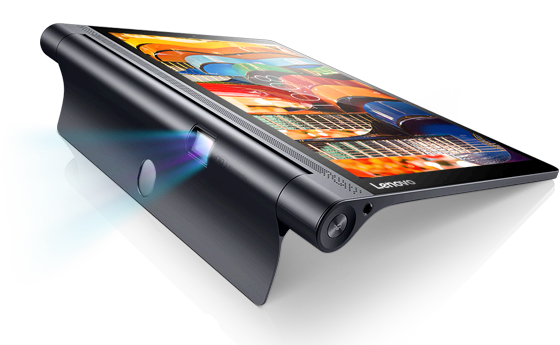
\includegraphics[width=0.38\linewidth]{Figures/lenovo_yoga_tab3_pro_front.png} 
  \caption{Moja prva slika}
  \label{slk:prvaslika}
\end{figure}

Referenciramo se na sliku \ref{slk:prvaslika} u sredini rečenice, zatim prije zareza \ref{slk:prvaslika}, te zatim na kraju rečenice \ref{slk:prvaslika}.
Upravo smo testirali radi li naredba \verb|\ref| ispravno u slučaju kada nakon nje slijedi točka.

Sada slijedi jedna jednadžba:
\begin{equation}
  \label{jed:prvajednadzba}
  \int_{-\infty}^{+\infty}f(t)\,dt=F(\omega)
\end{equation}
Jednadžba \eqref{jed:prvajednadzba} je moja prva jednadžba koja defnira par $f(t)\ufrek F(\omega)$ ili $F(\omega)\uvrem f(t)$.

%--- PRIVITCI / APPENDIX -------------------------------------------------------

% Sva poglavlja koja slijede će biti označena slovom i riječi privitak / All following chapters will be denoted with an appendix and a letter
\backmatter

\chapter{The Code}

\Blindtext


\end{document}
